\documentclass[../notes.tex]{subfiles}

\pagestyle{main}
\renewcommand{\chaptermark}[1]{\markboth{\chaptername\ \thechapter\ (#1)}{}}
\stepcounter{chapter}

\begin{document}




\chapter{???}
\section{Separable ODEs}
\begin{itemize}
    \item \marginnote{10/3:}Do not sit on the left side of the classroom: The sun sucks!
    \item \textbf{Separable} (ODE): An ODE of the form
    \begin{equation*}
        \dv{y}{t} = f(t)g(y)
    \end{equation*}
    where $y$ is a real\footnote{We'll deal with complex functions later.}, unknown, scalar function of $t$.
    \item Solving separable ODEs: Formally, evaluate
    \begin{equation*}
        \int\frac{\dd{y}}{g(y)} = \int f(t)\dd{t}
    \end{equation*}
    \item Rearrange the initial separable ODE to $\dv*{y}{t}\cdot 1/g=f$ and invoke the law of composite differentiation to get
    \begin{equation*}
        \dv{t}\left[ \int_{y_0}^{y(t)}\frac{\dd{w}}{g(w)}-\int_{t_0}^tf(\tau)\dd{\tau} \right] = 0
    \end{equation*}
    \item It follows that
    \begin{equation*}
        \int_{y_0}^{y(t)}\frac{\dd{w}}{g(w)} = \int_{t_0}^tf(\tau)\dd{\tau}
    \end{equation*}
    \item Examples:
    \begin{enumerate}
        \item Exponential growth.
        \begin{itemize}
            \item We have that
            \begin{equation*}
                \dv{y}{t} = ky
            \end{equation*}
            for $k>0$ and $y(0)=y_0>0$.
            \item The solution is
            \begin{align*}
                \frac{1}{y}\cdot\dv{y}{t} &= k\\
                \log y(t)-\log y_0 &= kt\\
                y(t) &= y_0\e[kt]
            \end{align*}
        \end{itemize}
        \item Logistic growth.
        \begin{itemize}
            \item We have that
            \begin{equation*}
                \dv{y}{t} = ky\left( 1-\frac{y}{M} \right)
            \end{equation*}
            for $k,M>0$ and $y(0)=y_0>0$.
            \item The solution is
            \begin{align*}
                \frac{M\dd{y}}{y(M-y)} &= k\dd{t}\\
                \log\frac{y}{M-y}-\log\frac{y_0}{M-y_0} &= kt\\
                \frac{y(M-y_0)}{y_0(M-y)} &= \e[kt]\\
                y\cdot\frac{M-y_0}{y_0} &= (M-y)\e[kt]\\
                y\cdot\frac{M-y_0}{y_0}+y\e[kt] &= M\e[kt]\\
                y\left( \frac{M-y_0}{y_0}+\e[kt] \right) &= M\e[kt]\\
                y\left( \frac{M-y_0+y_0\e[kt]}{y_0} \right) &= M\e[kt]\\
                y\left( \frac{M+y_0(\e[kt]-1)}{y_0} \right) &= M\e[kt]\\
                y(t) &= \frac{My_0\e[kt]}{M+y_0(\e[kt]-1)}
            \end{align*}
            \item Sketches the graph of logistic growth and discusses the turning point (for which there is a formula; zero of the second derivative) as well as general trends.
            \item If $y_0<0$, the solution is not physically meaningful, but it is mathematically insightful.
            \begin{itemize}
                \item When we integrate, the arguments of our logarithms now have absolute values.
                \begin{equation*}
                    \log\left| \frac{y}{M-y} \right|-\log\left| \frac{y_0}{M-y_0} \right| = kt
                \end{equation*}
                \item We need to make sure that the denominator of the final logistic form is never equal to zero, but now that $y_0$ is negative, as $t$ increases, the denominator will approach zero exponentially. It reaches zero when
                \begin{align*}
                    M+y_0(\e[kt]-1) &= 0\\
                    \e[kt] &= -\frac{M}{y_0}+1
                \end{align*}
                In other words, $t_\text{max}=(1/k)\log(1-M/y_0)$ because when $t=t_\text{max}$, the equation blows up.
                \item This is an example of \textbf{finite lifespan}.
            \end{itemize}
            \item If $y_0>M$, then you will exponentially decrease to $M$.
        \end{itemize}
        \item Lotka-Volterra predator-prey model.
        \begin{itemize}
            \item We have that
            \begin{align*}
                r' &= k_1r-awr&
                w' &= -k_2w+bwr
            \end{align*}
            where $r$ is rabbits and $w$ is wolves.
            \item We can rename the variables to
            \begin{equation*}
                \begin{cases}
                    x' = Ax-Bxy\\
                    y' = -Cy+Dxy
                \end{cases}
            \end{equation*}
            \item Dividing, we get
            \begin{align*}
                \frac{x'}{y'} &= \frac{Ax-Bxy}{-Cy+Dxy}\\
                \frac{By-A}{y}y'+\frac{Dx-C}{x}x' &= 0
            \end{align*}
            \item Use the fact that $x,y$ are independent variables, so both terms in the above equation are equal to zero?
            \item Invoke the law of composite differentiation twice and, from the above, know that $0+0=0$, so we can add the two solutions:
            \begin{align*}
                \dv{t}(By(t)-A\log y(t))+\dv{t}(Dx(t)-C\log x(t)) &= 0\\
                By(t)-A\log y(t)+Dx(t)-C\log x(t) &= E
            \end{align*}
            \item Sketches some of the trajectories (they're all closed curves in the $xy$-plane).
            \begin{figure}[h!]
                \centering
                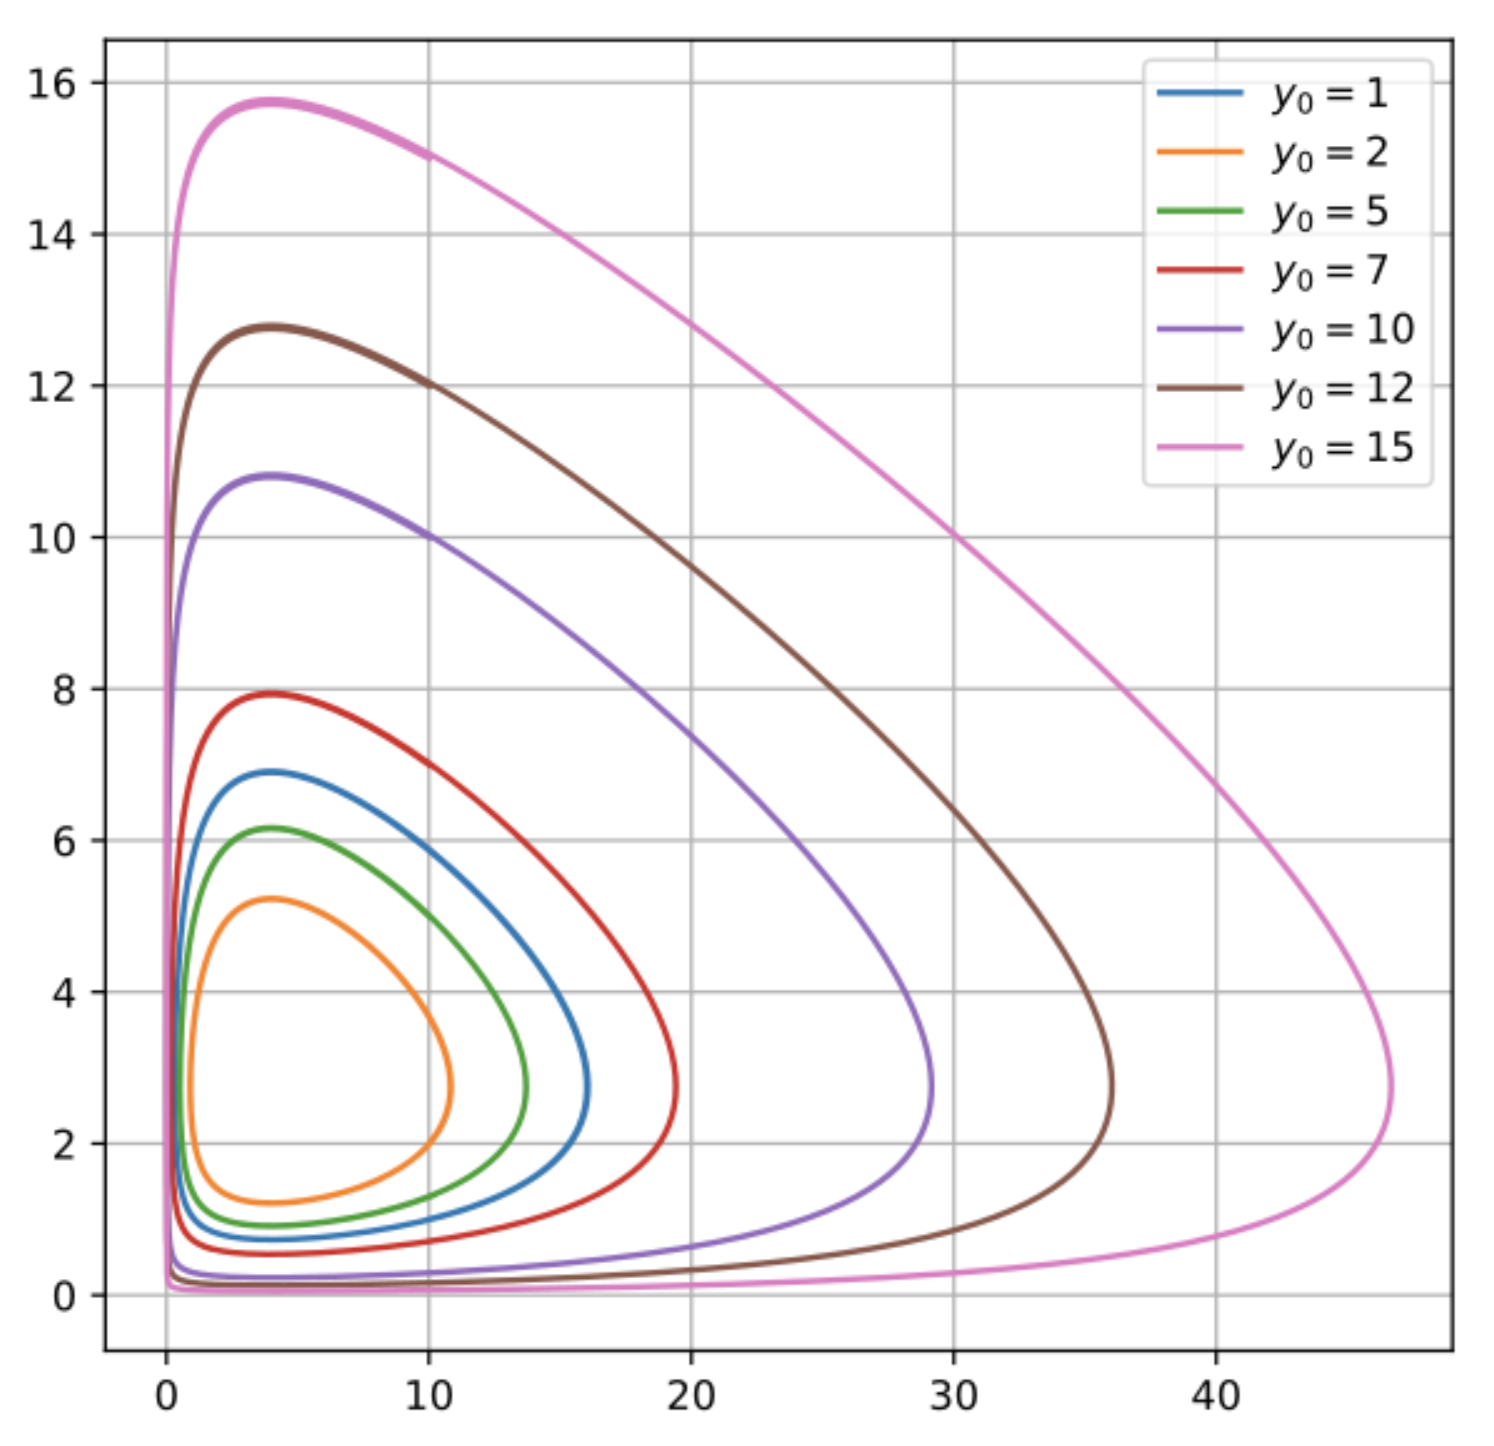
\includegraphics[width=0.4\linewidth]{../ExtFiles/LotkaVolteraSolns.png}
                \caption{Lotka-Volterra solution curves.}
                \label{fig:LotkaVolteraSolns}
            \end{figure}
            \item Properties of the curves:
            \begin{itemize}
                \item The implicit relation which determines them: By the implicit function theorem, the $y$ derivative of the LHS is $B-A/y$ and the $x$-derivative of the LHS is $D-C/x$. When the partial derivatives are equal to zero, $(C/D,A/B)$ becomes interesting. Turning points happen when the $y$-coordinate is $A/B$ or the $x$-coordinate is $C/D$.
            \end{itemize}
        \end{itemize}
    \end{enumerate}
    \item \textbf{Finite lifespan}: Even if the RHS of $\dv*{y}{t}=f(t,y)$ is very regular, the solution can still blow up at some finite time.
    \item Consider the following variation on the E-L equation from the Brachistochrone problem.
    \begin{equation*}
        \dv{y}{x} = \sqrt{\frac{B-y}{y}}
    \end{equation*}
    \begin{itemize}
        \item Finding the \textbf{primitives}.
        \begin{itemize}
            \item What are these "primitives" Shao keeps talking about?
        \end{itemize}
        \item We should have
        \begin{equation*}
            \int\sqrt{\frac{y}{B-y}}\dd{y} = x
        \end{equation*}
        \item Change of variables: $y=B\sin^2\phi$ and $\dd{y}=2B\cos\phi\sin\phi\dd{\phi}$. Thus,
        \begin{equation*}
            \int\sqrt{\frac{y}{B-y}}\dd{y} = \int\frac{\sin\phi}{\cos\phi}\cdot 2B\cos\phi\sin\phi\dd{\phi}
            = 2B\int\sin^2\phi\dd{\phi}
        \end{equation*}
        \item The solution is
        \begin{equation*}
            \begin{cases}
                x = B\phi-\frac{B}{2}\sin(2\phi)+C\\
                y = B\sin^2\phi
            \end{cases}
        \end{equation*}
        \begin{itemize}
            \item This is a parameterization of a cycloid.
        \end{itemize}
    \end{itemize}
    \item Later in the week, we will do the SHM, the pendulum, the Kepler 2-body problem, and the Michaelis-Menten equation.
    \item Separable ODEs are a subset of ODEs of \textbf{exact form}.
    \item ODEs of exact form are of the form
    \begin{equation*}
        g(x,y)\dv{y}{x}+f(x,y) = 0
    \end{equation*}
    where for some $F(x,y)$, $g=\pdv*{F}{y}$, $f=\pdv*{F}{x}$, and partials commute. Equivalently,
    \begin{equation*}
        \pdv{g}{x} = \pdv{f}{y}
    \end{equation*}
    is our necessary and sufficient condition.
    \item By the law of composite differentiation,
    \begin{align*}
        \dv{x}\left[ F(x,y(x)) \right] &= \pdv{F}{x}(x,y(x))+\pdv{F}{y}(x,y(x))\cdot y'(x)\\
        &= f(x,y(x))+g(x,y(x))y'(x)\\
        &= 0
    \end{align*}
    \begin{itemize}
        \item We solve these with an integrating factor $\mu\neq 0$ such that $(\mu g,\mu f)$ satisfy the constraint.
    \end{itemize}
\end{itemize}



\section{Office Hours (Shao)}
\begin{itemize}
    \item \textbf{Primitive}: An antiderivative.
    \item \textbf{Law of composite differentiation}: The chain rule.
    \item Went over how Shao has been applying the law of composite differentiation with respect to separable ODEs:
    \begin{itemize}
        \item Rearrange the initial separable ODE as follows.
        \begin{equation*}
            \frac{1}{g(y)}\cdot\dv{y}{t} = f(t)
        \end{equation*}
        \item Define $\dv*{H}{y}=1/g(y)$. Then, continuing from the above, we have by the law of composite differentiation that
        \begin{align*}
            \dv{H}{y}\cdot\dv{y}{t} &= f(t)\\
            \dv{H}{t} &= f(t)
        \end{align*}
        \item From the definition of $H$, we know that $H(y)=\int_{y_0}^y\dd{w}/g(w)$. We also have from the FTC that $f(t)=\dv{t}\int_{t_0}^tf(\tau)\dd{\tau}$. Thus, continuing from the above, we have that
        \begin{align*}
            \dv{t}(H) &= f(t)\\
            \dv{t}\left[ \int_{y_0}^y\frac{\dd{w}}{g(w)} \right] &= \dv{t}\int_{t_0}^tf(\tau)\dd{\tau}\\
            \dv{t}\left[ \int_{y_0}^{y(t)}\frac{\dd{w}}{g(w)}-\int_{t_0}^tf(\tau)\dd{\tau} \right] &= 0
        \end{align*}
        as desired.
        \item It follows since $y(t_0)=y_0$ that $C=H(y_0)=0$, so we can take the above to
        \begin{equation*}
            \int_{y_0}^{y(t)}\frac{\dd{w}}{g(w)} = \int_{t_0}^tf(\tau)\dd{\tau}
        \end{equation*}
        knowing that our constant of integration is zero.
    \end{itemize}
    \item Take away from Brachistochrone problem: Just an example of a BDE; we won't have to answer questions on it.
\end{itemize}



\section{ODEs of Exact Form}
\begin{itemize}
    \item \marginnote{10/5:}Last time, we discussed separable ODEs.
    \item Today, we will study \textbf{exact form} equations, as discussed last class.
    \item \textbf{Exact form} (ODE): An ODE of the form
    \begin{equation*}
        g(x,y)\dv{y}{x}+f(x,y) = 0
    \end{equation*}
    where
    \begin{equation*}
        \pdv{g}{x} = \pdv{f}{y}
    \end{equation*}
    \item For equations of this form, there exists $F(x,y)$ such that
    \begin{align*}
        \pdv{F}{x} &= f&
        \pdv{F}{y} &= g&
        F(x,y(x)) &= C
    \end{align*}
    for some $C\in\R$.
    \item To solve equations of this form, we need an \textbf{integrating factor}.
    \item \textbf{Integrating factor}: A number or function $\mu$ such that
    \begin{align*}
        \mu g\dv{y}{x}+\mu f &= 0&
        \pdv{x}(\mu g) &= \pdv{y}(\mu f)
    \end{align*}
    \item For linear homogeneous equations $\dv*{y}{t}=p(t)y$, we have
    \begin{equation*}
        y(t) = y_0\exp[\int_{t_0}^tp(\tau)\dd\tau]
    \end{equation*}
    \item Recall that $\e[a+ib]=\e[a](\cos b+i\sin b)$, so
    \begin{align*}
        \e[ix] &= \cos x+i\sin x&
        \cos x &= \frac{1}{2}(\e[ix]+\e[-ix])&
        \sin x &= \frac{1}{2i}(\e[ix]-\e[-ix])
    \end{align*}
    \item Example: If $y'=ky$, then $y'=-\lambda y$.
    \item If we have an inhomogeneous linear equation $\dv*{y}{t}=p(t)y+f(t)$, then
    \begin{equation*}
        \dv{y}{t}-py-f = 0
    \end{equation*}
    but
    \begin{equation*}
        0 = \dv{t}(1) \neq \dv{y}(-p(t)y-f(t))
    \end{equation*}
    \item We wish to find an integrating factor $\mu(t,y)$ such that
    \begin{equation*}
        \mu(t,y)\dv{y}{t}-\mu(t,y)p(t)y-\mu(t,y)f(t) = 0
    \end{equation*}
    and
    \begin{equation*}
        \dv{t}(\mu) = \dv{y}(-\mu py-\mu f)
    \end{equation*}
    \item Solution: Take $\mu$ to be a function of $t$, alone. Then
    \begin{equation*}
        \mu'(t) = \dv{y}(-\mu py-\mu f) = -\mu(t)p(t)
    \end{equation*}
    and we now have a homogeneous linear equation with solution
    \begin{equation*}
        \mu(t) = \exp[-\int_{t_0}^tp(\tau)\dd\tau]
    \end{equation*}
    \begin{itemize}
        \item If we let $P(t)=\int_{t_0}^tp(\tau)\dd\tau$, then
        \begin{align*}
            \e[-P(t)]y'(t)-p(t)y(t)\e[-P(t)] &= \e[-P(t)]f(t)\\
            \dv{t}(\e[-P(t)]y(t)) &= \e[-P(t)]f(t)\\
            \e[-P(t)]y(t) &= \int_{t_0}^t\e[-P(\tau)]f(\tau)\dd\tau
        \end{align*}
        \item Thus, we finally have the solution to the inhomogeneous problem as follows: The IVP $y'=py+f$, $y(t_0)=y_0$ has solution
        \begin{equation*}
            y(t) = y_0\e[P(t)-P(t_0)]+\e[P(t)]\int_0^t\e[-P(\tau)]f(\tau)\dd\tau
        \end{equation*}
        where $P$ is any anti-derivative of $p$.
    \end{itemize}
    \item In particular, when $p(t)=a$, we get the \textbf{Duhamel formula} (which we should memorize).
    \item \textbf{Duhamel formula}: The following equation, which is the solution to an inhomogeneous linear equation with $p(t)=a$.
    \begin{equation*}
        y(t) = y_0\e[a(t-t_0)]+\int_{t_0}^t\e[a(t-\tau)]f(\tau)\dd\tau
    \end{equation*}
    \begin{itemize}
        \item Important for computing forced oscillation.
    \end{itemize}
    \item Inspecting the inhomogeneous solution.
    \begin{itemize}
        \item The first term is the solution to the homogeneous form. The second term deals with the initial value.
    \end{itemize}
    \item Given an inhomogeneous equation, you can always write its solution as the combination of the solution to the homogeneous problem plus a particular solution, i.e.,
    \begin{equation*}
        y = y_h+y_p
    \end{equation*}
    \begin{itemize}
        \item "The general solution equals the homogeneous solution plus a particular solution."
        \item This is related to linear algebra, where the solution to $Ax=b$ is a particular solution $x_p$ plus any vector $x\in\ker A$.
        \item Thus, this idea will reappear in the theory of systems of linear ODEs.
    \end{itemize}
    \item We now look at systems of linear ODEs.
    \item Consider the harmonic oscillator: A particle of mass $m$ connected to an ideal spring (obeys Hooke's law) with no friction or gravity.
    \begin{itemize}
        \item Newton's second law: The acceleration is proportional to the restoring force.
        \item Hooke's law: The restoring force is of magnitude $kx$ in the opposite direction to the displacement.
        \item Thus, the ODE is of the form
        \begin{equation*}
            x'' = -\frac{k}{m}x
        \end{equation*}
    \end{itemize}
    \item Consider an ODE of the form
    \begin{equation*}
        y''+ay'+by = 0
    \end{equation*}
    for $a,b\in\C$.
    \begin{itemize}
        \item Aim: Find $\mu,\lambda\in\C$ such that
        \begin{equation*}
            (y'-\mu y)'-\lambda(y'-\mu y) = 0
        \end{equation*}
        \item To find the parameters, we expand the above to
        \begin{equation*}
            y''-(\mu+\lambda)y'+\mu\lambda y = 0
        \end{equation*}
        \item Comparing with the original form, we have that $a=-(\mu+\lambda)$ and $b=\mu\lambda$.
        \item It follows that $\mu,\lambda$ are the roots of $x^2+ax+b=0$, which we will call the \textbf{characteristic polynomial} of the ODE.
    \end{itemize}
    \item Example:
    \begin{itemize}
        \item Consider
        \begin{equation*}
            y'-\mu y = A\e[\lambda t]
        \end{equation*}
        \item By the Duhamel equation, we have that a particular solution is of the form
        \begin{equation*}
            A\int_0^t\e[\mu(t-\tau)]\e[\lambda\tau]\dd\tau
        \end{equation*}
        \item Thus, general solutions are of the form
        \begin{equation*}
            y(t) = B\e[\mu t]+C\e[\mu t]\int_0^t\e[(\lambda-\mu)\tau]\dd\tau
        \end{equation*}
        \item Evaluating the integral, we get
        \begin{equation*}
            y(t) = B\e[\mu t]+C\e[\mu t]\frac{\e[(\lambda-\mu)t]-1}{\lambda-\mu}
        \end{equation*}
        which simplifies (by incorporating constants, etc.) to
        \begin{equation*}
            y(t) = A_1\e[\mu t]+B_1\e[\lambda t]
        \end{equation*}
        for $\mu\neq\lambda$, or
        \begin{equation*}
            y(t) = A_1\e[\mu t]+B_1t\e[\mu t]
        \end{equation*}
        for $\mu=\lambda$.
    \end{itemize}
    \item If our equation is of the form $y''+ay'+by=f(t)$, then we just need to apply the Duhamel formula twice.
    \item Returning to the simple harmonic oscillator problem, we substitute $\omega=\sqrt{k/m}$ to get
    \begin{equation*}
        x'' = \omega^2x
    \end{equation*}
    \begin{itemize}
        \item The characteristic polynomial is
        \begin{equation*}
            0 = x^2+\omega^2
            = (x+i\omega)(x-i\omega)
        \end{equation*}
        \item Thus, solutions are of the form
        \begin{equation*}
            x = A_1\e[i\omega t]+B_1\e[-i\omega t]
        \end{equation*}
        \item It follows that the period is $T=2\pi/\omega$.
        \item To get a real (usable) solution, apply Euler's formula to get
        \begin{align*}
            x(t) &= A_1(\cos\omega t+i\sin\omega t)+B_1(\cos\omega t-i\sin\omega t)\\
            &= A\cos\omega t+B\sin\omega t
        \end{align*}
        where $A=A_1+B_1$, $B=iA_1-iB_1$.
        \item To match the initial condition $x(0)=x_0$, $x'(0)=v_0$, we use
        \begin{equation*}
            x(t) = x_0\cos\omega t+\frac{v_0}{\omega}\sin\omega t
        \end{equation*}
        \item In other words,
        \begin{align*}
            &
            \begin{cases}
                A=x_0\\
                \omega B=v_0
            \end{cases}
            &&
            \begin{cases}
                A_1+B_1=x_0\\
                i\omega A_1-i\omega B_1=v_0
            \end{cases}
        \end{align*}
        so
        \begin{align*}
            &
            \begin{cases}
                A=x_0\\
                B=\frac{v_0}{\omega}
            \end{cases}
            &&
            \begin{cases}
                A_1=\frac{1}{2}\left[ x_0-\frac{iv_0}{\omega} \right]\\
                B_1=\frac{1}{2}\left[ x_0+\frac{iv_0}{\omega} \right]
            \end{cases}
        \end{align*}
    \end{itemize}
\end{itemize}




\end{document}